\documentclass{Template_resources/netsci-project}

% :::~ This is the configuration for the bibliography. DO NOT CHANGE
\usepackage[
    backend=biber,
    style=authoryear,
    natbib=false,
    maxcitenames=2,
    minbibnames=1, maxbibnames=99, 
    url=false, 
    doi=true,
    ]{biblatex}
\addbibresource{References/references.bib}
\usepackage{verbatim}
\usepackage{hyperref}
\usepackage{caption}
\usepackage{subcaption}

\begin{document}
\firstpage{1}
\subjectarea{Blockchain \& Distributed Ledger Technologies}
\title{Final Project - Epidemic spreads over the flight network}
\author{Marlene Funke (15-738-719), Aleksandar Novković (16-733-032), Sandra Trachsel (15-718-190), Miguel Vázquez (16-712-598)}
\course{Network Science}
\school{Faculty of Business, Economics and Informatics}
\date{December 19th, 2022}
\maketitle

%%%%%%%%%%%%%%%%%%%%%%%%%%%%%%%%%%%%%%%%%%%%%%%%%%%%%%%%%%%%%%%%%%%%
%%%%%%%%% ABSTRACT
%%%%%%%%%%%%%%%%%%%%%%%%%%%%%%%%%%%%%%%%%%%%%%%%%%%%%%%%%%%%%%%%%%%%

\begin{abstract}
This project analyzes possible scenarios for a pandemic spreading in the global airport network. By simulating the pandemic with a SIR-model we aim to rank different centrality measures in terms of how well they identify which airports to close first in an effort to reduce damage and spread of a next potential pandemic. Our findings imply that the best measure depends on which outcome you care about the most.
\end{abstract}

%%%%%%%%%%%%%%%%%%%%%%%%%%%%%%%%%%%%%%%%%%%%%%%%%%%
%%%%%%%%% INTRODUCTION
%%%%%%%%%%%%%%%%%%%%%%%%%%%%%%%%%%%%%%%%%%%%%%%%%%%%%%%%%%%%%%%%%%%%

\section{Introduction}
Globalization and technology growth have connected people around the world like never before. One of the examples is the increase in fast and reliable human transportation networks such as the World Airline Network (WAN). Nevertheless, with increasing levels (both in terms of frequency and reach) of human mobility also comes increasing risk of a quick spread of infectious diseases: epidemics.\footnote{Throughout the paper we will be using ``pandemic'' and ``epidemic'' interchangeably due the difficulty of drawing a line when running simulations.} In practical comparison, during the Covid-19 pandemic, we could observe similar phenomena. Hospitals were often overloaded, because there were very high waves in the outbreak of the infection. This is crucial to analyze; decisive policy actions appear essential by seeing how skyrocketing the disease spreads at the beginning of the outbreak, in such a short amount of time.

In our paper we want to test if we can use five centrality measures (betweenness, eigenvector, closeness, in-degree and out-degree) to properly identify and shut down spreader nodes as to avoid a new pandemic taking over. In particular, we are interested in how these measures rank at identifying such nodes, under different levels of government allowance (i.e. how many airports can be actually shut down). For this purpose, we use a Susceptible-Infected-Recovered (SIR) model to simulate the spread of a pandemic through the WAN. 

We will focus on the following questions: is there a definite best centrality measure to achieve the above mentioned goal? If yes, which one (of the ones we selected) is it? If no, why so? Does it depend on the outcome?

We will start by shortly discussing the existing literature on the topic, followed by a description of the assumptions that we made in our model. Next, in the data and methods section, we will describe the raw data, the data preparation and the procedure of our analysis. This will be followed by the results description and discussion. A concluding statement rounds out the paper.

%%%%%%%%%%%%%%%%%%%%%%%%%%%%%%%%%%%%%%%%%%%%%%%%%%%%%%%%%%%%%%%%%%%%
%%%%%%%%% THEORY
%%%%%%%%%%%%%%%%%%%%%%%%%%%%%%%%%%%%%%%%%%%%%%%%%%%%%%%%%%%%%%%%%%%%

\section{Theory}
\subsection{Literature}
The rapid spread of the new Coronavirus has caused huge social and economic damage around the world. One of the biggest concerns for pandemics is globalization and the fast and frequent movement of individuals across the world. The World Airline Network (WAN) has heavily increased the speed and scope of human mobility, and with it, it has created an efficient transmission channel for infectious diseases, allowing pandemics to spread more rapidly around the world (\cite{Lawyer2016}). International passenger numbers increased from 1.67 Billion in 2000 to 2.63 Billion in 2010 and an astonishing 4.56 Billion in 2019, just before the COVID-19 pandemic forced down 2020's numbers back to 2005 levels (\cite{WorldBank}).

\cite{Morse2012} explain that the frequency of new emerging pathogens is also increasing over time, with most of these viruses originating in animals and infecting humans due to behavioural, socioeconomic and economical changes. Only in the last few decades we have witnessed the emergency of HIV, Ebola Virus Disease, SARS, H1N1 influenza, MERS-CoV and other novel zoonotic diseases. All of these are affecting people and crossing the geopolitical boundaries of nation-states (\cite{MartinBoland2018}). \cite{Balcan2009}, and \cite{Brockmann2013} both support this conclusion with observational studies of influenza; nevertheless, this is also supported by studies of other epidemics like malaria (\cite{Hunag2013}) and dengue fever (\cite{Semanza2014}).

The topological structure of the WAN is well characterized. The network is a scale-free small-world one, with a strong community structure that is imposed by spatial constraints (\cite{Lawyer2016, Barrat2005}). \cite{Verma2014} use a similar WAN. They find that their WAN is divided into three parts:
69.41\% of the airports serve as bridges that connect a heavily interconnected core of the 2.26\% major transportation hubs (72 airports) to peripheral airports and regional population centres (28.33\%). For a passenger to travel between any pair of airports, it needs at most to go through 12 connections. However, on average, 33\% of the routes can be covered with at most three connections.
Since actual outcomes of arising infectious diseases are critically shaped by chance events in early stages of their emergence, it is important to understand clearly how seed location can influence global outcomes. This could improve public health planning significantly (\cite{Lawyer2016}). 
This WAN allows us to rationalize the role of its large-scale properties within the predictability and heterogeneity of an epidemic pattern (\cite{Colizza2006TheMO}).

\subsection{Centrality measures}
In our analysis we will use a SIR-model where we test if we can use five centrality measures (betweenness, eigenvector, closeness, in-degree and out-degree) to identify spreader nodes and so avoid a new pandemic by shutting down those airports. 

The betweenness centrality (BC) calculates the shortest paths between all pairs of nodes in a graph. It has the power to identify bottlenecks within the network, i.e. an airport with high BC may not have the most directed connections to other airports, but serves as a bridge to these which are very well connected. These airports have more control over the flow of spreading through the network, because there is no other airport that is better positioned. Thus, the global spread of a disease could be limited by closing such airports.

Closeness centrality (CC) measures the shortest distance of a node to all other nodes. Nodes with high CC are therefore able to reach other nodes more easily. We chose this measure with the assumption that airports with the highest CC are the main sources of disease transmission, as they spread it very efficiently across the network. We hypothesize this might be the most important centrality measure in our analysis since it is a topologically meaningful concept of centrality within networks when it comes to spreading. 

The eigenvector centrality (EC) assigns a relative value to a node with respect to the nodes it is connected to. Thus a node connected to another node with more importance always receives a higher centrality value. For example, large airports, with many connections (e.g. Paris Charles de Gaulle (CDG) in France), are more important than those connected to smaller airports that do not have many connections to others (e.g. like on Saba in the Caribbean Islands (SAB)). 

We also wanted to take a measure of degree centrality (DC) but since we have a directed network, we selected both in-degree (IC) and out-degree (OC) centralities. The in-degree is the number of flights arriving, and the out-degree is the number of flights leaving the airport. This means that the importance of an airport is measured by the number of arrivals and departures to or from other airports and therefore have a greater impact on the global spread of the disease.

%%%%%%%%%%%%%%%%%%%%%%%%%%%%%%%%%%%%%%%%%%%%%%%%%%%%%%%%%%%%%%%%%%%%

\subsection{Model assumptions}
To begin with our analysis, we had to make some assumptions. Firstly, we assume that in our network, the nodes represent airports and not people or passengers; additionally, all the airports have the same weight. On the other hand, the edges of our network represent (directed) routes between airports. We weighted those edges by the number of airlines on that route $\times$ the number of seats on the plane type that the airline uses for that route, following \citeauthor{Lawyer2016}'s (\citeyear{Lawyer2016}) approach. We are thus assuming that the airline's plane type decision for a given route is not random but rather a proxy of the connection's importance and its demand. During our data preparation, we also assumed that the same aircraft models have the same number of seats, and since all flight data was recovered from OpenFlights, we have no reason to believe that they would include cargo-shipping routes in their database. Furthermore, we assume that there is only one flight per route and period.

We use a standard Susceptible-Infected-Recovered (SIR) model defined as a continuous-time Markov chain (CTMC). We arbitrarily fix the recovery rate at 0.5 and the infection rate at 0.005, since for our exercise we simply need these rates to be constant to achieve a ceteris paribus environment. We select a quite high recovery rate because we want the epidemic to die out within our time limits, so that we are able to measure outcomes such as epidemic length. A further assumption is that some regulation exists allowing us to completely shut down any airport and all of its routes and that the selected airports will cancel all their flights simultaneously. 
Finally, we arbitrarily fix the share of initially randomly infected nodes at 0.5\%. In this way, we can reflect on the delay between the emergence of the virus and the action taken by governments. Moreover, it reduces the likelihood of trivial epidemics, where only the initial infected node(s) are infected by the end as no transmission occurs.

%%%%%%%%%%%%%%%%%%%%%%%%%%%%%%%%%%%%%%%%%%%%%%%%%%%%%%%%%%%%%%%%%%%%
%%%%%%%%% METHODS
%%%%%%%%%%%%%%%%%%%%%%%%%%%%%%%%%%%%%%%%%%%%%%%%%%%%%%%%%%%%%%%%%%%%

\section{Data and methods}
\subsection{Raw data description}
We download raw data directly from the GitHub repository behind the OpenFlights.org website (\cite{OpenFlights2008}), only fetching the \textit{airports.dat}, \textit{routes.dat}, and \textit{planes.dat} databases. The length of the airports database is 7,697 (after we drop 1 erroneous non existing airport) and observations are uniquely identified by either OpenFlights' own airport ID or the airport's International Civil Aviation Organization (ICAO) 4-digit code, since the International Air Transport Association airport (IATA) 3-digit code is missing for 1,625 airports. On the other hand, the length of the routes database is 67,663 and observations are uniquely identified by the combination of the airline code, departure airport IATA code and arrival airport IATA code. This means that, originally, any two nodes might be connected by multiple edges. Finally, the length of the airplanes database is 246 and observations are uniquely identified by the airplane name.

%%%%%%%%%%%%%%%%%%%%%%%%%%%%%%%%%%%%%%%%%%%%%%%%%%%%%%%%%%%%%%%%%%%%

\subsection{Data preparation}
From the routes database we only keep departure and arrival airport codes as well as the plane types used, allowing us to generate a WAN with the help of the NetworkX package (\cite{networkx}). We then match the network nodes with the airports database to retrieve the airports' geographical coordinates. We find out that 3,260 out of 3,422 (95\%) unique IATA codes from the routes dataset are also present in the airports dataset. Out of the remaining 162 unmatched airports, we are able to fix 29 of them by manually imputing the missing IATA code variable in the airports database.\footnote{In particular, 25 are airports/heliports in Greenland and the remaining 4 are airports each in one of the following countries: China, Iran, Russia, United States.} We drop the remaining unmatched 133 nodes (summing up to 497 edges) as we believe they are not included in the airports database.\footnote{While manually imputing the IATA codes where possible, we realize that the vast majority of the 133 unmatched codes are airports in Alaska, United States. This should not pose a big issue of representativity since it appears from Figure \ref{fig:final_network} that already quite many airports in Alaska are included in the network.} Finally, 5 nodes remain now isolated so we also drop them. This process results in a edge loss of around 0.75\% compared to the original network: we end up with 3,284 hubs and 67,148 connections.

We proceed with the preparation of our network by adding weights to the edges. For this purpose, we follow the approach used in \citeauthor{Lawyer2016} (\citeyear{Lawyer2016}) meaning that edges are weighted based on the number of seats of the carrier used for a given connection. After matching the plane types on the routes database with the planes database, we use WorldTrading.net to get flight capacity estimates for the different airplane types via web-scraping. For several aircrafts (specially Airbus and Boeing) it seems like different codes are used to identify the same model of aircraft, but with e.g. different engine. We use SeatLink.com to find out if two airplane types are the same model and unify the number of seats. We do the same for the 4 aircrafts which are labeled as \textit{cargo} on WorldTrading.net. Finally, we impute the seats for the remaining missing airplane types by manually looking for the aircraft on Wikipedia.org or, when not available, on SeatGuru.com.\footnote{Note that in the planes database the IATA codes \textit{CN1} and \textit{CNJ} are given as reference for multiple different aircrafts. Since we cannot know exactly which aircraft is being used in those cases we take the average of the seats across all different aircrafts that were merged to that code. In particular, we assign 5 seats to \textit{CN1}, and 8 seats to \textit{CNJ}.}

The final step of the data preparation involves simplifying the network from a parallel multi-edge directed one to a simple directed one with at most two edges between any two nodes. Here again we follow the approach used in \citeauthor{Lawyer2016} (\citeyear{Lawyer2016}), where they multiply the weight of each edge by the number of parallel edges between the two nodes. With this last step we are reducing the number of edges by 45\% such that at the end of the whole data preparation process we have 3,284 nodes and 37,189 edges. Figure \ref{fig:final_network} shows graphically the scale and complexity of the network that we will be analysing.
\begin{figure}[!h]
    \centering
    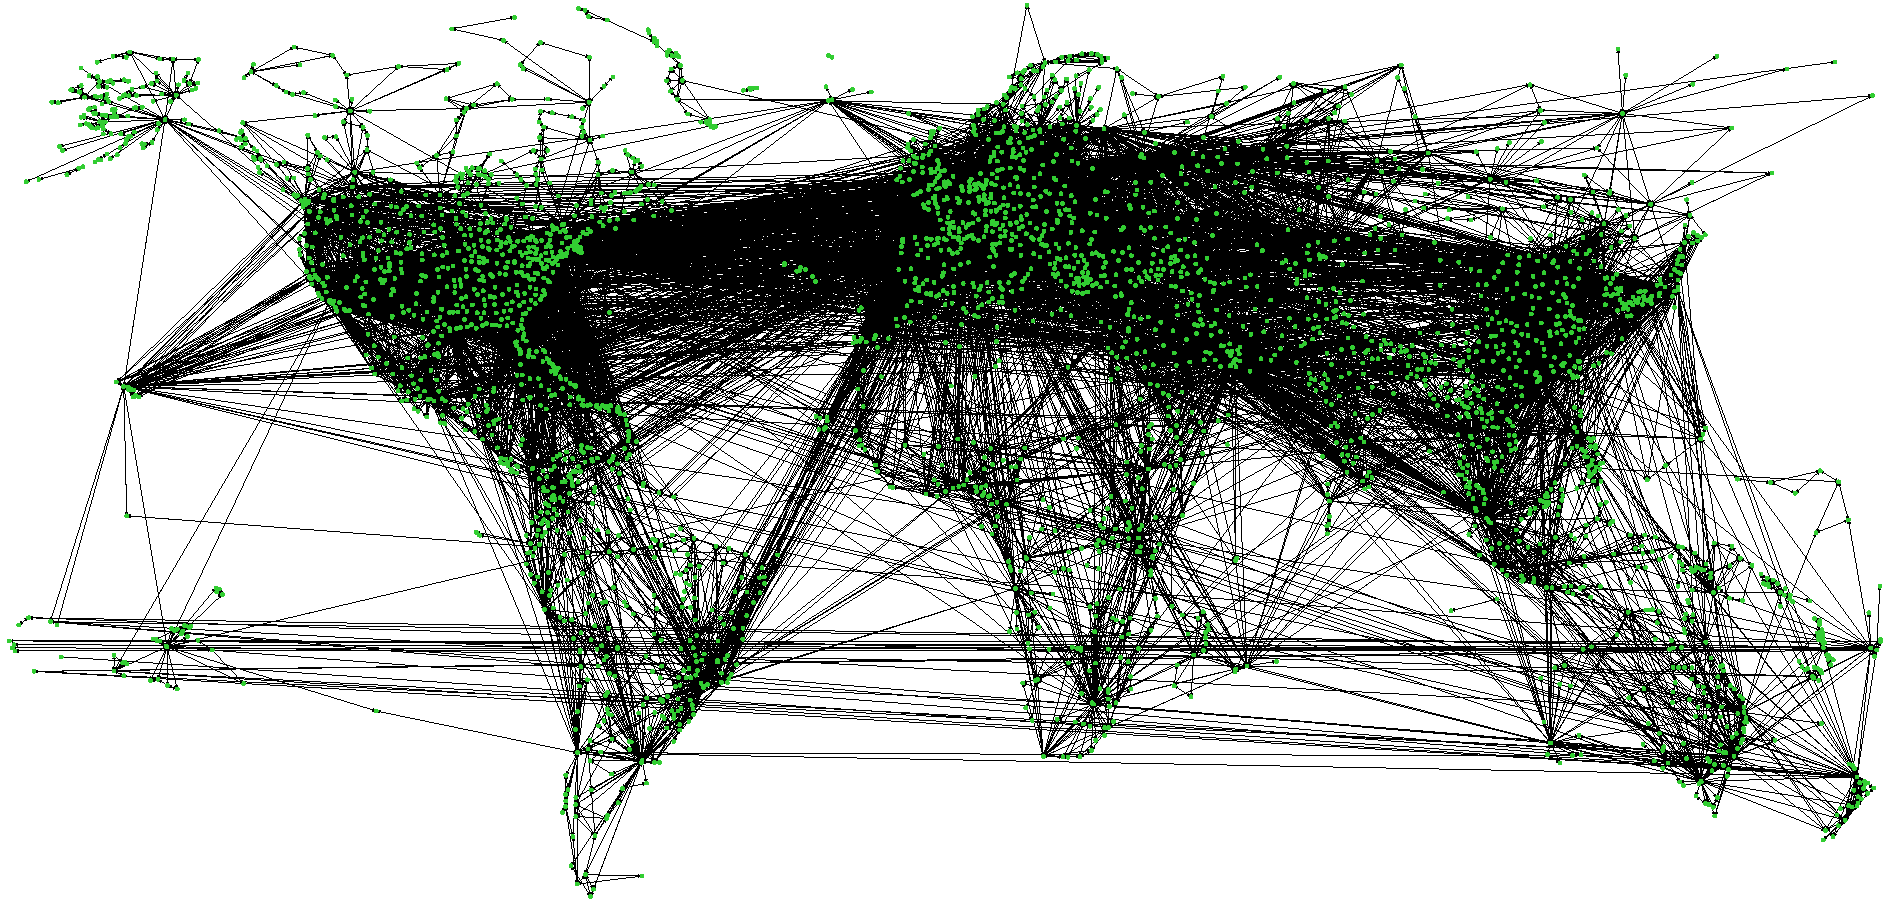
\includegraphics[width=\linewidth]{Figures/final_network.pdf}
    \caption{Visual representation of the flight network covered by our data.}
    \label{fig:final_network}
\end{figure}

%%%%%%%%%%%%%%%%%%%%%%%%%%%%%%%%%%%%%%%%%%%%%%%%%%%%%%%%%%%%%%%%%%%%

\subsection{Analysis}
Our analysis consists of running simulations for a spreading disease using the Epidemics on Networks (EoN) library (\cite{eon}). EoN simulates the spread of a disease in a network by solving an Ordinary Differential Equation (ODE) model as we have seen it in class. In order to obtain plausible and consistent solutions for the ODE-model, the number of iterations has to be set high enough. This number depends on the characteristics of the baseline network at hand and we found 100 to be good enough for us. The specific ODE-model used in this analysis is the SIR-model which solves three differential equations for each component of the model (S-,I-,R-equation) with respect to t (time-points in the simulation) simultaneously. Through this iterative solving of the equation system we get dynamically rich simulations which are mainly driven by parameters that are specified in the model: transmission rate of the infection (which is individual for each edge as it gets enhanced by the edge weights), recovery rate of infected nodes, share of randomly initial infected nodes, and the $t$-max parameter which limits the number of periods for which the spread should be simulated.

Due to the high number of simulations that we intended to run, including initial experiments and robustness checks, we decided to use the $fast\_SIR$ module in order to keep the computation times low. Furthermore, the $fast\_SIR$ is rather a simple form of the SIR-model, since it simulates for constant and exponentially distributed infection and recovery rates, which are determined by the user. For a wider analysis of spreading diseases there is a variety of different simulation functions in the EoN package, which allow the user more detailed specifications about the parameters, such as inserting functions for the transmission instead of a singular rate. For the purpose of generality and simplicity we decided to analyze the airport network using only the most simple SIR-model. Furthermore, implementing the much more complicated simulations would go far beyond the scope of this work without adding substantial contribution to the main question of this analysis.

One crucial problem we had in the beginning was that the $fast\_SIR$ simulation returned very inconsistent arrays of time steps, and thus all the outcomes, due to the continuous nature of the system solution mechanism. Since we need to align all the simulations in order to calculate averages and standard errors, we needed the $t$-steps to be uniform (or at least consistent). For this purpose we used linear interpolation with small steps (one tenth of $t$) to recover uniform information on the number of infected nodes for all of our simulations. In Figure \ref{fig:interpolation_test} one can observe optically one example of reconstructing the simulated epidemic courses using linear interpolation. 
\begin{figure}[!h]
    \centering
    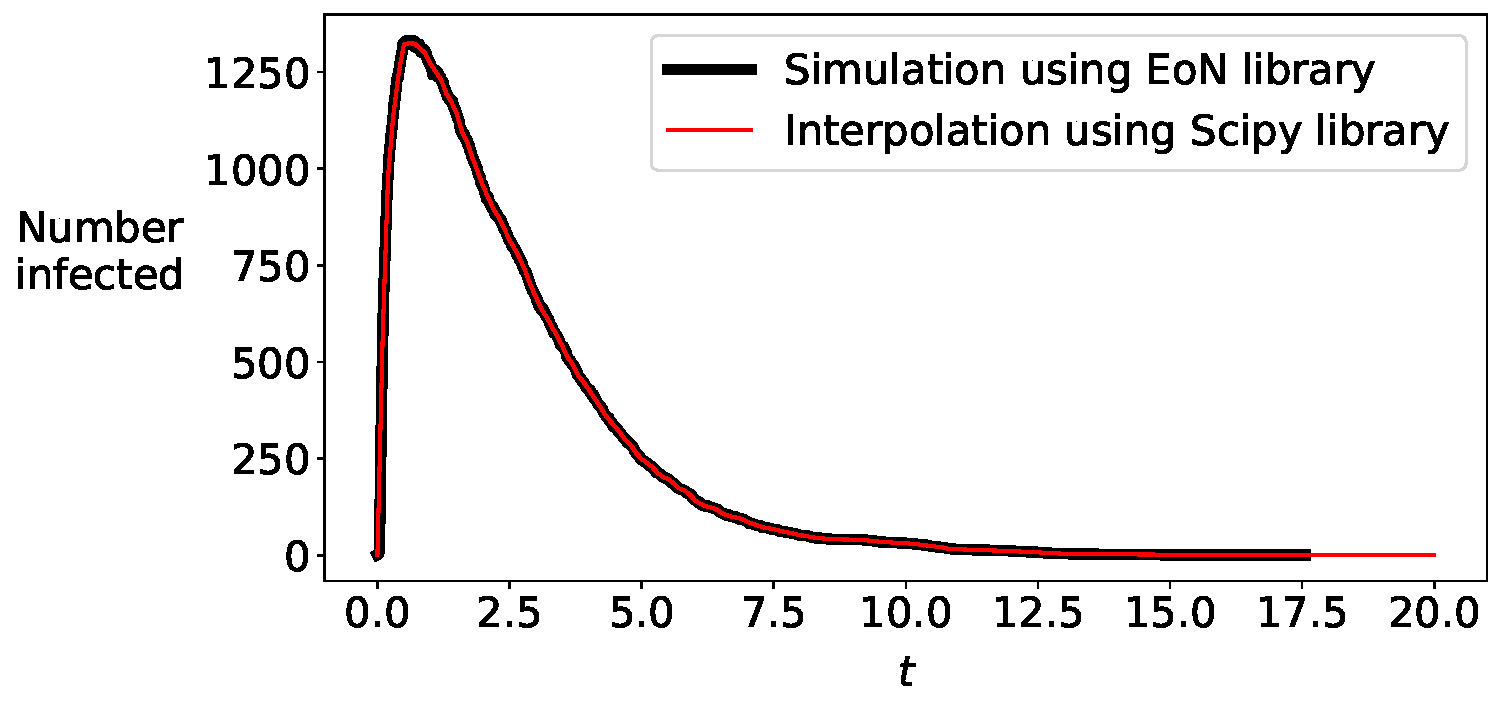
\includegraphics[width=0.5\linewidth]{Figures/interpolation_test.pdf}
    \caption{One example of simulated epidemic course interpolation using SciPy's \href{https://docs.scipy.org/doc/scipy/reference/interpolate.html}{interpolate subpackage}. Note that we force infected numbers to be equal to 0 from the moment the epidemic dies until our defined $t$-max parameter (i.e. 20).}
    \label{fig:interpolation_test}
\end{figure}

After settling on the simulation specifications we created the different counterfactual networks necessary for our analysis. For each of our five selected centrality measures we defined groups of the top 1\% to 12\% highest ranked nodes for each measure individually and create a copy of the network where we shut down the nodes in those groups. It is important to note that we \emph{did} not remove the airports from the WAN altogether, but rather simply removed the edges. This is consistent with the idea that these nodes are eligible by nature to be initially infected. We thus end up with 60 scenarios of protective measures in addition to the baseline one. The size of the groups is differentiable invasive, since the top 1\% nodes are equivalent to ``only'' 33 nodes, while the top 12\% represents 394 nodes. We then ran 100 simulations for each centrality measure plus the baseline for each of the topX\% groups, and then computed averages and standard errors across them for four different outcomes of interest: height of peak, total number of infected people, time until peak and total pandemic length. 

As mentioned earlier the baseline parameter selection was quite arbitrary. We expected that variations in this sense would not change the dynamics of the simulation in terms of relative ranking for the centrality measure, but rather only change the absolute sizes of the outcomes: e.g. a higher peak if the transmission rate is ceteris paribus higher, or alternatively, a longer pandemic if the recovery rate is higher. To be sure we performed some robustness checks that could confirm our hypothesis which is crucial for our analysis, since it makes our findings robust for all reasonable combinations of the parameters within the simulation. In particular, we tested all combinations between three different transmission rates (0.1, 0.2 and 0.4) and recovery rates (0.1, 0.2 and 0.3) on the number of infections at the peak of the epidemic. This also allowed us to experiment with values of the basic reproduction rate $R_0$ both above and below 1. As we had expected the relative ranking of the centrality did not seem to be affected by the parameter selection as it remained constant across all combinations and equal to the case where the parameters take the values stated in the assumptions.


%%%%%%%%%%%%%%%%%%%%%%%%%%%%%%%%%%%%%%%%%%%%%%%%%%%%%%%%%%%%%%%%%%%%
%%%%%%%%% RESULTS
%%%%%%%%%%%%%%%%%%%%%%%%%%%%%%%%%%%%%%%%%%%%%%%%%%%%%%%%%%%%%%%%%%%%

\section{Results and discussion}
%%%% Spearman matrix
The first question that comes to mind when performing this exercise is how much the five selected centrality measures correlate. Figure \ref{fig:measure_comparison} seeks to help us gain insight on this. Subfigure \ref{fig:spearman_matrix} plots a matrix of Spearman's rank correlation coefficients. It can be seen that the EC and CC measures yield very similar rankings of the nodes in our network. This can be interpreted by saying that the airports closest to all others are almost congruent with those that have the property of being connected to many nodes that themselves have high connectivity to others. The same is true for the rankings of the IC and OC measures, which is reasonable since we expect airports with many inbound flights also to have many outbound flights. On a similar fashion, Subfigure \ref{fig:node_remove_overlap_matrix} shows a weighted average of the share of nodes that overlap among the topX\% sets. Though the Subfigures appear similar, it is noticeable that the EC and CC correlations are not that high from a different angle.
\begin{figure}[!h]
    \begin{subfigure}[t]{0.5\textwidth}
        \centering
        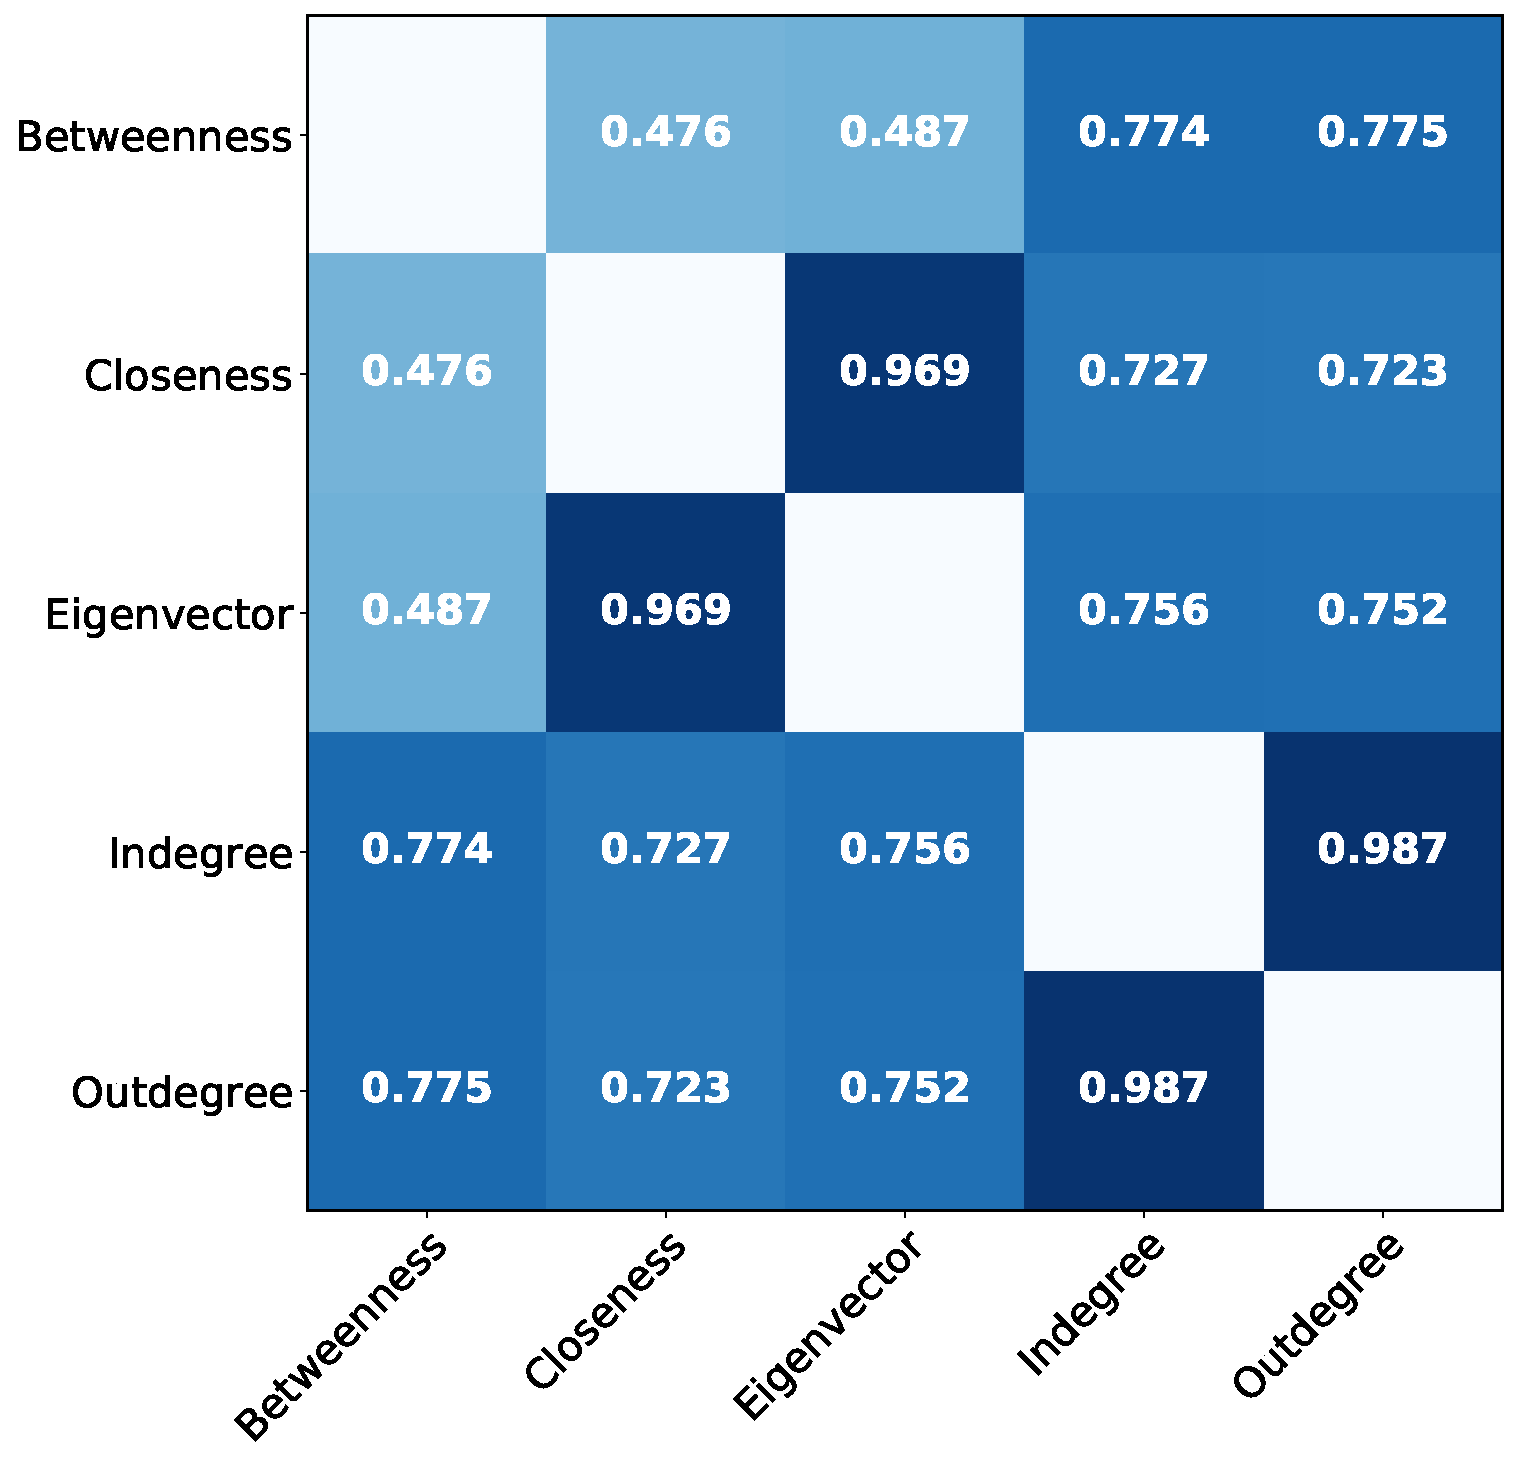
\includegraphics[width=\linewidth]{Figures/spearman_matrix.pdf}
        \caption{\raggedleft Spearman's rank correlation coefficient matrix.}
        \label{fig:spearman_matrix}
    \end{subfigure}
    \hfill
    \begin{subfigure}[t]{0.5\textwidth}
        \centering
        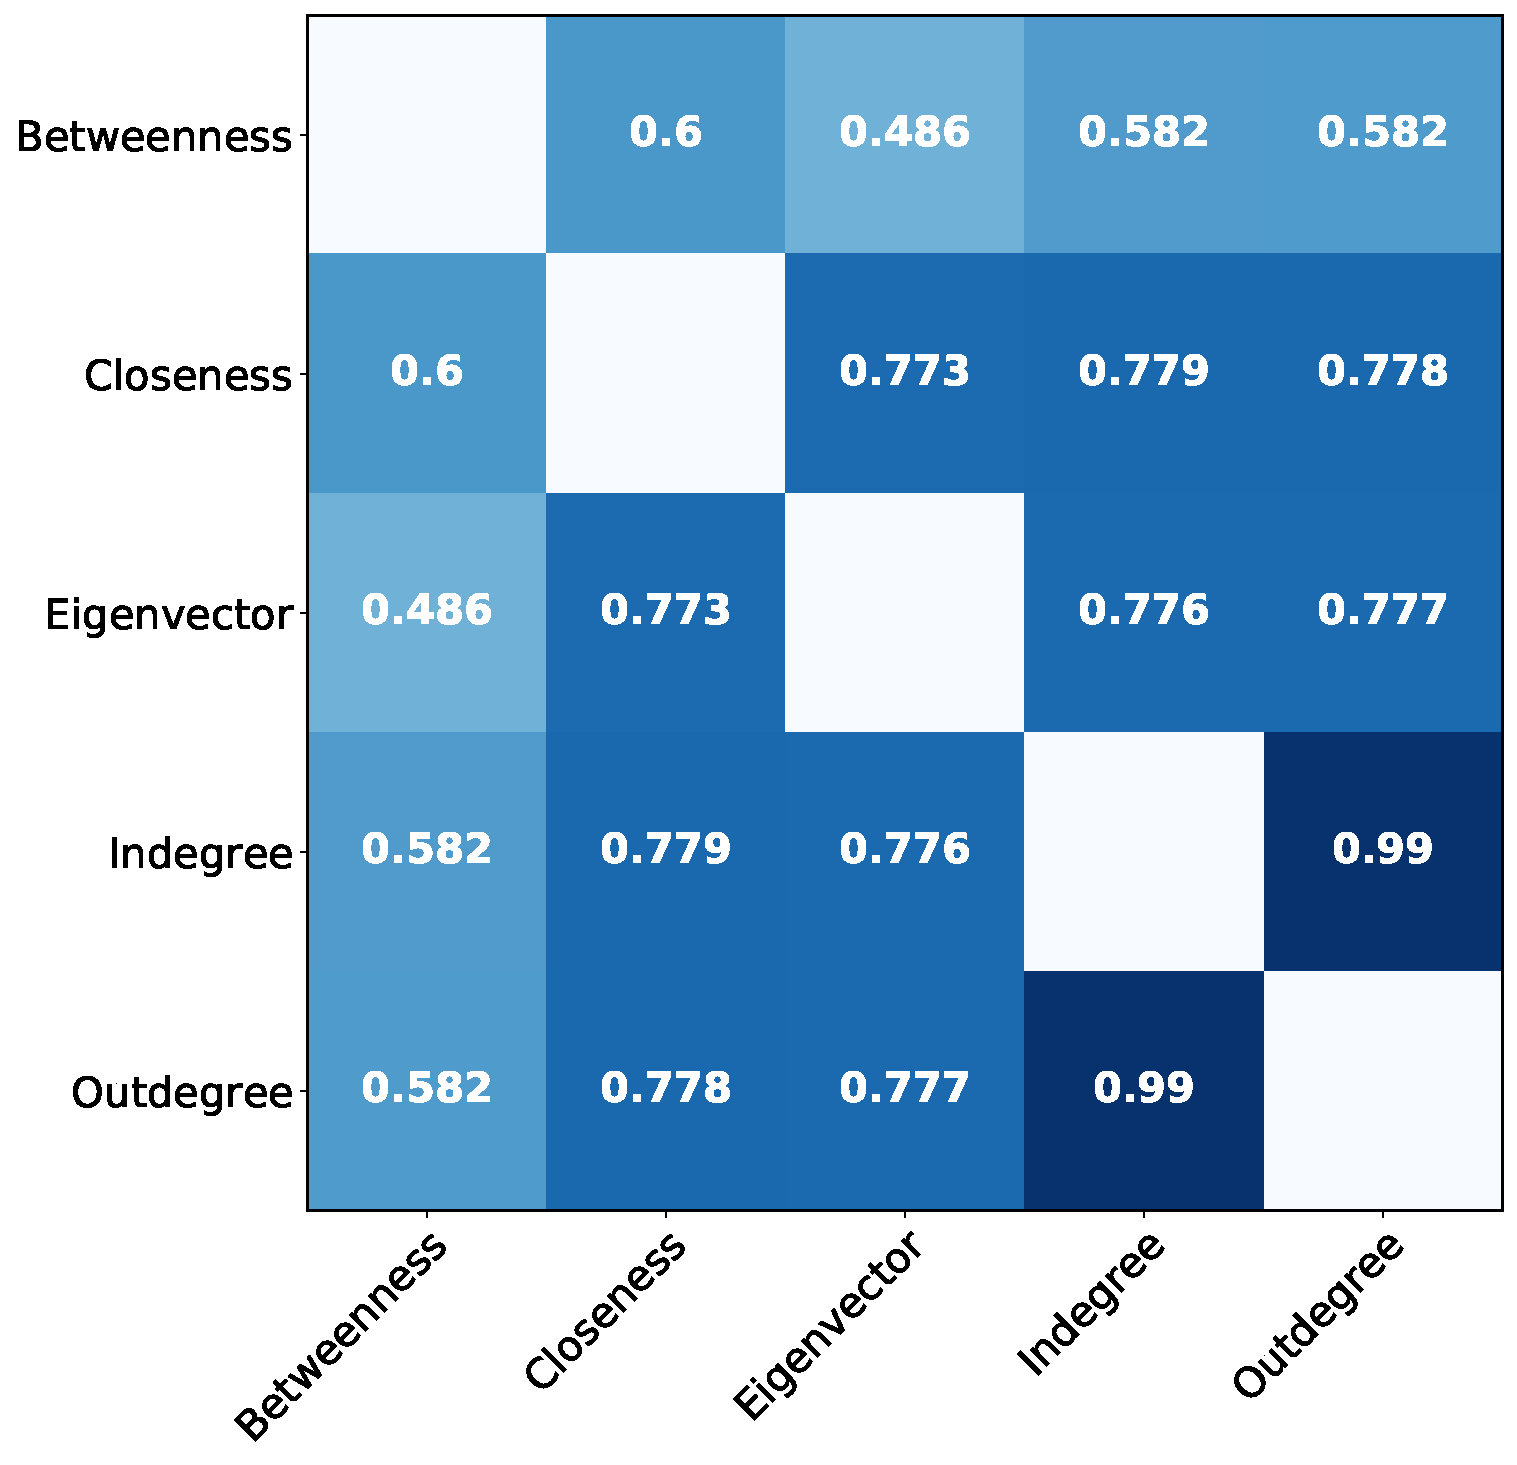
\includegraphics[width=\linewidth]{Figures/node_remove_overlap_matrix.pdf}
        \caption{\raggedleft Weighted average (by the number of nodes being removed) of the share of nodes that overlap among the topX\% sets of each two measure combination.}
        \label{fig:node_remove_overlap_matrix}
    \end{subfigure}
    \caption{Comparing centrality measures}
    \label{fig:measure_comparison}
\end{figure}


%%%% Outcomes of interest
In Figure \ref{fig:interest_outcomes} we want to take a closer look at the effects of shutting down selected nodes on our outcomes of interest, namely peak of epidemic, entirety of epidemic, time until peak and epidemic length.
\begin{figure}[!h]
    \centering
    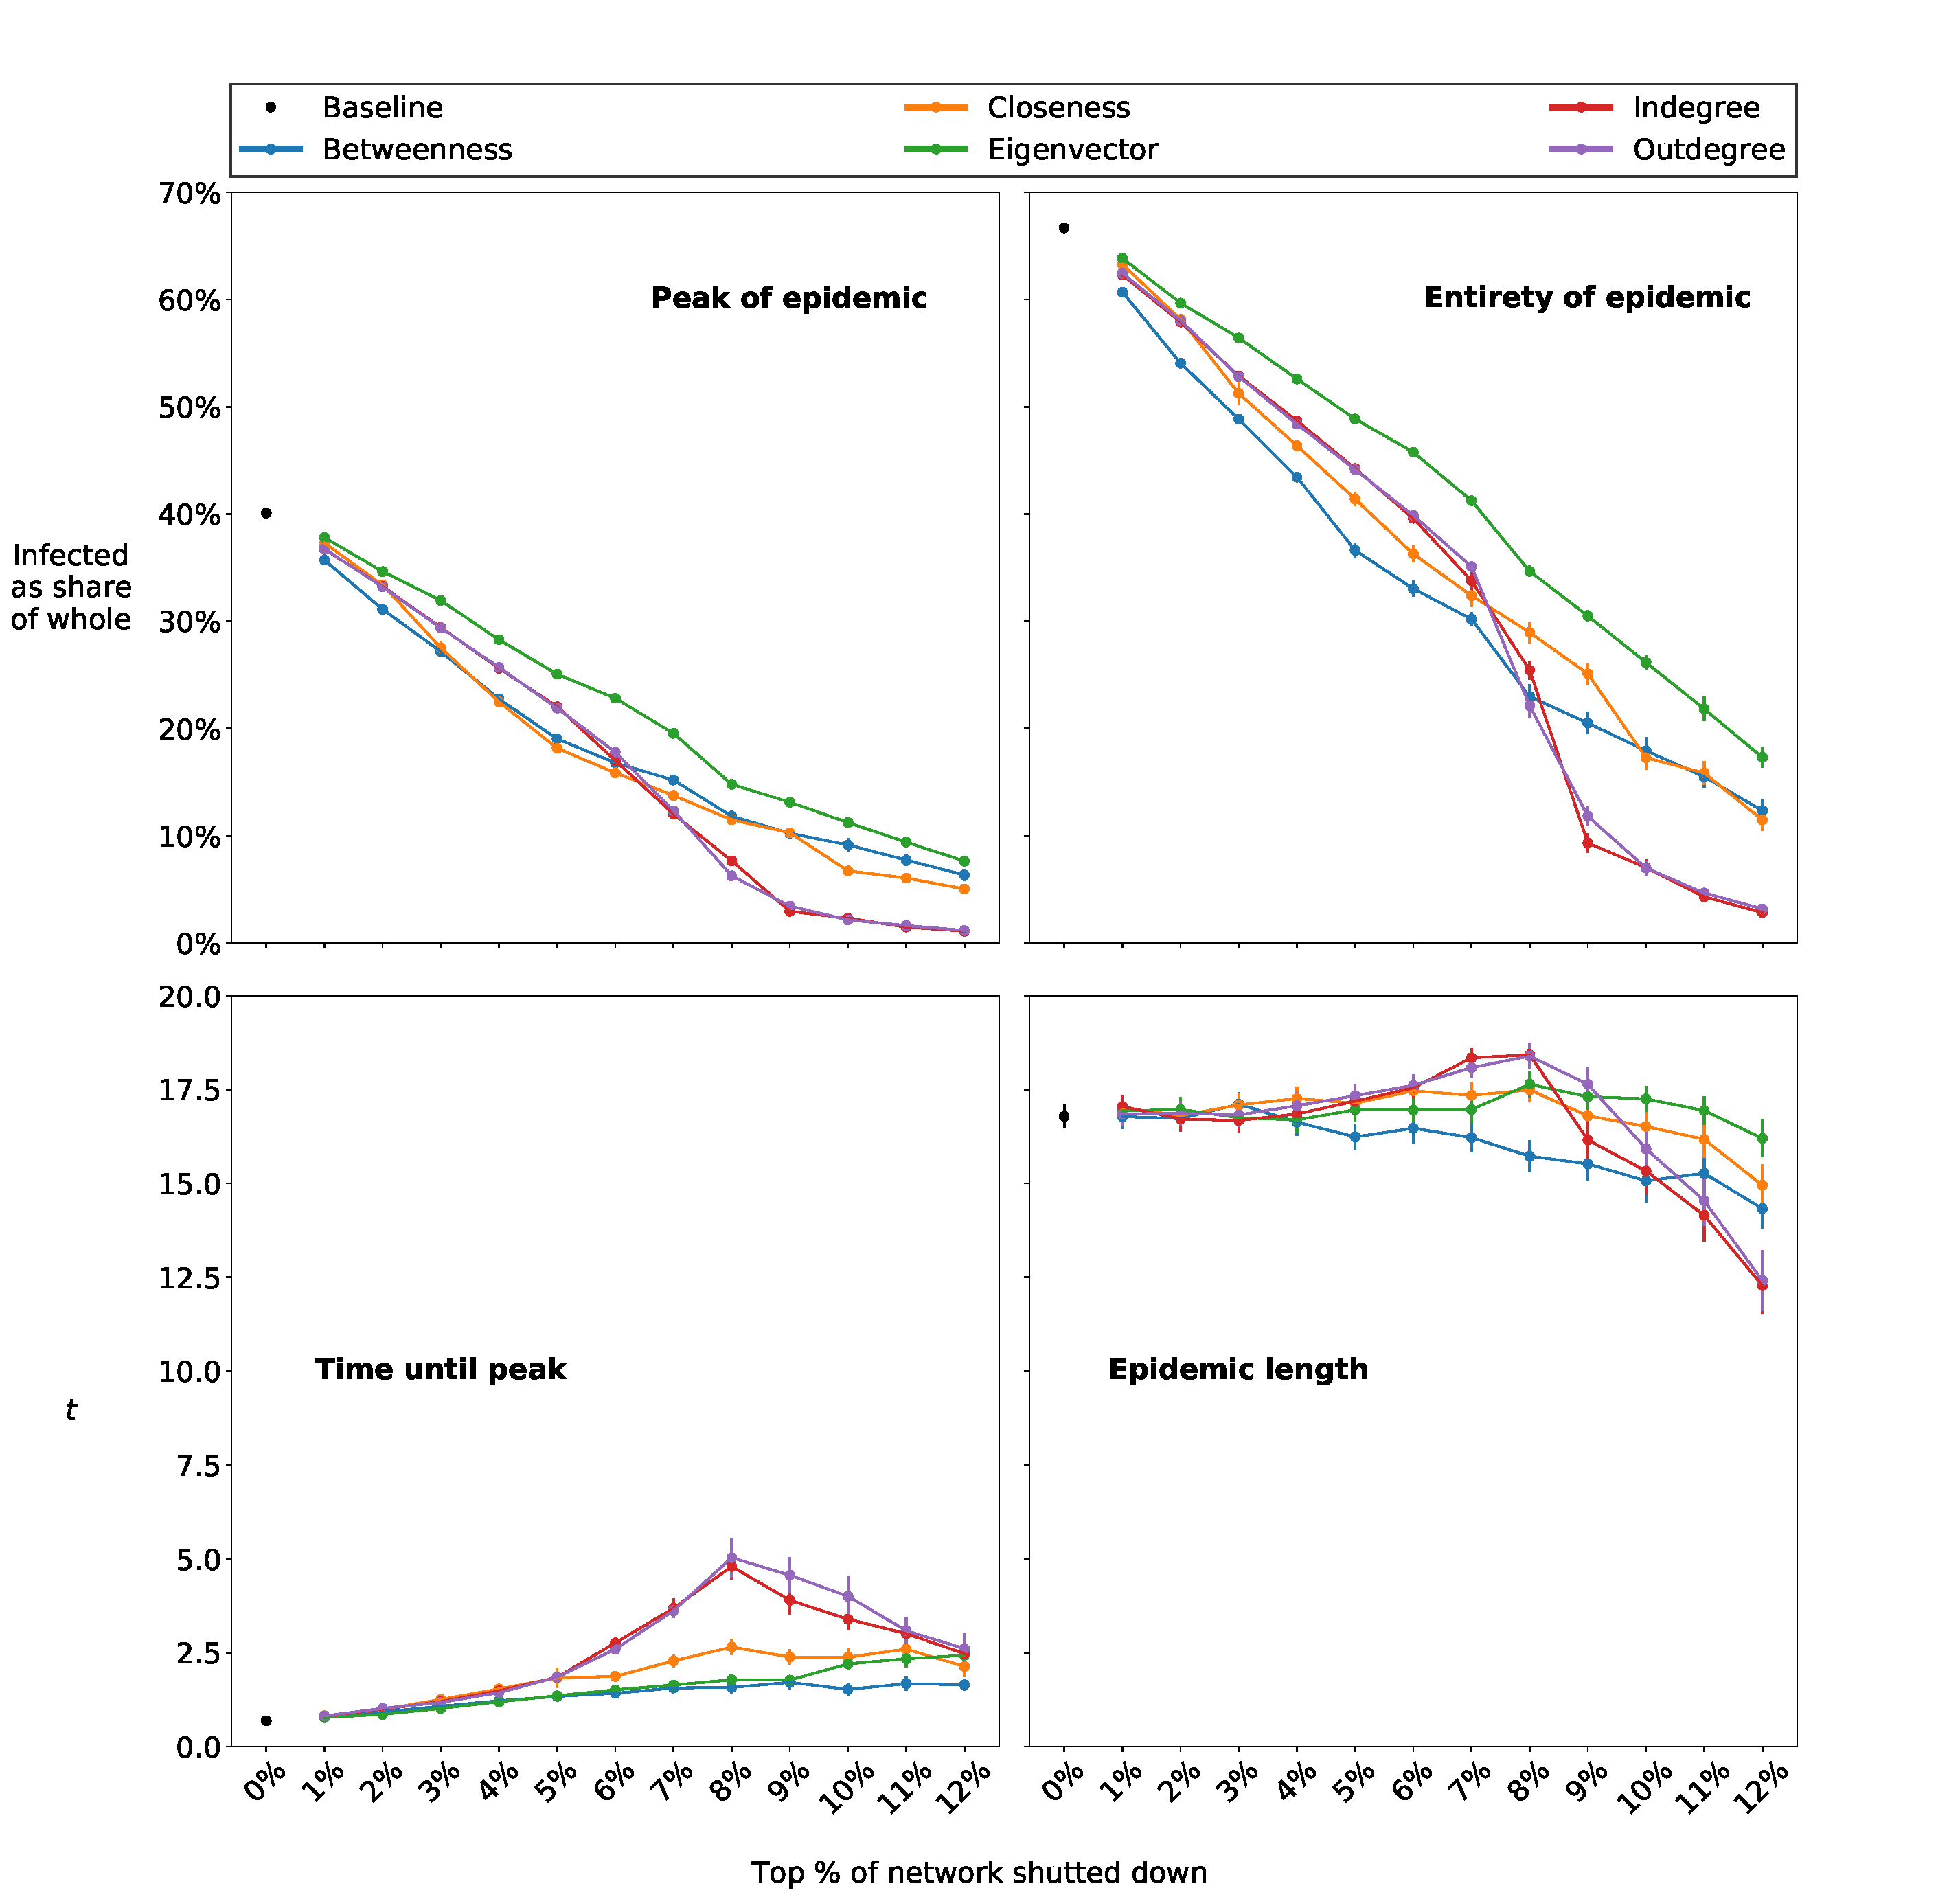
\includegraphics[width=\linewidth]{Figures/interest_outcomes.pdf}
    \caption{Depicted are the effects of selected nodes' shutting down through edges removal on four different outcomes of interest.}
    \label{fig:interest_outcomes}
\end{figure}

\textbf{Peak of epidemic}. We see that in the baseline model, at most 40\% of the nodes were infected simultaneously at the peak. By looking at the centrality measures removing the top 1\% most central nodes, between 30\% and 40\%  of total nodes were infected at the peak. We see a sharp drop in the rate of infected nodes as more important nodes are removed. Removing 12\%  of the top nodes decreases the rate of infected nodes at the peak below 10\%  for all centrality measures. For the DC even down to almost 0\%. It is interesting that the BC and CC reach a smaller peak than the DC up to a distance of 6\% of the nodes, but after that a much flatter course can be observed and thus take on values more like those of the EC, while the DC continue to drop sharply in their peaks' height.

\textbf{Entirety of epidemic}. We can note that the base model records 70\% infected nodes. Again, we see a very similar trend of the infection rate as before as more important nodes are removed, with the number of infected nodes dropping to below 20\%.  However, a much steeper drop is noted here. It is interesting to see that we can spot a quite similar effect where after a certain degree of allowance DC measures overtake the others.

\textbf{Time until peak}. Starting from the baseline model, we notice that we reach the peak extremely quickly, as the infected nodes are skyrocketing. From the baseline model we can observe a minimal increasing trend up to about 5\%, the more important nodes are removed, i.e. the cases of infection increase in a slower pace so to reach the peak it takes longer. The DC are an exception, the time to peak slows down drastically, by about twice the time compared to the other measures at a removal of 8\% of the most important nodes, but drops from there on to similar values as the other centrality measures.

\textbf{Epidemic length}. Starting from the baseline model we see an overall slightly decreasing trend. The EC shows a fairly constant trend, i.e. there is hardly any change. For the BC and CC we see that the length of the epidemic course is somewhat reduced. The DC are a special case, which is related to the time to peak observations. First, the epidemic length increases until the 7\% of the most important nodes are reduced, followed by a very strong reduction of the length as more nodes are extracted, finally reaching the shortest length of the epidemic course.\\


To come back to our stated questions from the introductory part; in order to describe the best strategy for a successful political measure to be introduced, with our underlying method to remove topX\% central ranked nodes, we need to state which requirement is needed to see a pandemic as successfully contained. This results from the fact, that different centrality measurements resume in different containment-strategies, thus it depends whether we want to minimize the peak of the pandemic, the entirety of the pandemic, the time until the pandemic peaks or its overall length. 

Depending on the stage of the pandemic in the real world as well as the economic state and the critical situation of the healthcare systems, different strategies should be taken into account. It is evident that stronger safety measures indicate a stronger flattering of the pandemic. However, these safety measures are closely tied to economical costs and omission of economical activities, which form a significant social trade-off between the newly infected in a population and the monetary costs and losses which result from the safety measures. 
%peak of pandemic
The prior made assumption, that the CC measure would be the most effective, cannot be made for all above stated dimensions of pandemic-indicators. It is, the most effective (together with BC) when it comes to reducing the peak of the pandemic, at least until the point of where 6\% of the top airports have been closed. From there on, if it's economically feasible to close more airports, the DC measurements seem to perform way better in terms of the total infections at the peak. 
%entirety of pandemic
In order to contain the entirety of the pandemic, which corresponds to the share of overall infected, and to restrict only a minimum of air traffic, it is recommended to close airports after the BC measurement (closing up to top 8\% of airports). The DC method is essential when we consider the closure of a larger proportion of airports. 
%epidemic length
When it comes to the whole epidemic length, the BC is again, the most suitable one. DC becomes important to consider if we were able to close a larger percentage of airports (shutting off up to top 9\% of the network).
%time until the pandemic peaks
Considering the time until the peak of the pandemic, which we want to be as high as possible so that we have time to plan and take certain measures thoughtfully, the DC method is clearly always to be preferred.

Resuming from the above stated properties, it seems like we can summarize our findings to two measurements which should be preferred in the containment of a pandemic: The BC and the DC. Especially when identifying and removing the first topX\% nodes, which are the most important ones in the network, the BC delivers the best results. When it comes to further-extending safety measures, which follow the closing of less important airports, the DC seem to identify the remaining structure by importance better than the remaining measures in this analysis.
These findings are further confirmed when analyzing Figure \ref{fig:spearman_matrix}. It can clearly be observed, that the correlation between the through DC and BC removed nodes is rather low compared to the other measurements. This aligns with the finding, that these two preferred centrality-measures are able to identify complementary nodes, which resume in different effects when following the aim to contain an ongoing pandemic. 



%%%%%%%%%%%%%%%%%%%%%%%%%%%%%%%%%%%%%%%%%%%%%%%%%%%%%%%%%%%%%%%%%%%%
%%%%%%%%% CONCLUSION
%%%%%%%%%%%%%%%%%%%%%%%%%%%%%%%%%%%%%%%%%%%%%%%%%%%%%%%%%%%%%%%%%%%%
\section{Conclusion}

In conclusion, we can clearly identify some patterns for an efficient containment from Figure \ref{fig:interest_outcomes} for the global spread of a disease corresponding to different safety measures.
It should be noted that there is not only one recommendation for everything. As discussed in the section above; diverse centrality measures are recommended, depending on the dimensions of pandemic-indicators we are looking at and factors such as the state of the pandemic, the economic situation and the occupancy rate of the health care system. 

In summary, if limited by economic factors, only a small number of airports can be closed, it is essential to consider the BC. However, if the health care system is overburdened and a higher number of airports, due to further-extending safety measures, need to be closed, DC should be taken into consideration in determining airport closures to most effectively contain a pandemic. We observe these different effects of the two different centrality measures because they identify partly complementary airports as important ones. 


%

%%%%%%%%%%%%%%%%%%%%%%%%%%%%%%%%%%%%%%%%%%%%%%%%%%%%%%%%%%%%%%%%%%%%
%%%%%%%%% REFERENCES
%%%%%%%%%%%%%%%%%%%%%%%%%%%%%%%%%%%%%%%%%%%%%%%%%%%%%%%%%%%%%%%%%%%%

\clearpage
\printbibliography

%%%%%%%%%%%%%%%%%%%%%%%%%%%%%%%%%%%%%%%%%%%%%%%%%%%%%%%%%%%%%%%%%%%%
%%%%%%%%% AUTHOR CONTRIBUTIONS
%%%%%%%%%%%%%%%%%%%%%%%%%%%%%%%%%%%%%%%%%%%%%%%%%%%%%%%%%%%%%%%%%%%%

\section*{Author contributions}
All authors conceived and designed the project idea, and defined the abstract. M. Vázquez prepared the data and curated the data analysis and deriving figures. S. Trachsel curated and wrote the ``Introduction'' and ``Theory'' sections. A. Novković curated and wrote the ``Data and methods'' and the ``Conclusion'' sections. M. Funke curated and wrote the ``Result and discussion'' section. All authors revised and accepted the final version of this document. All authors prepared and presented the slides.
\end{document}